In order to illustrate the complexities present in synthetic homotopy groups we will compute the bigraded groups $\pi_{k,*}(\nu_{\HFt} \Ss^{\wedge} _2)$ in the Toda range ($k \leq 19$).
We will see that these groups reflect the entire structure of the $\HFt$-Adams spectral sequence for $\Ss^{\wedge} _2$, including hidden extensions.
For brevity, throughout this section $\pi_{a,b}$ will refer to $\pi_{a,b}(\nu_{\HFt} \Ss^\wedge_2)$.

The $\HFt$-Adams spectral sequence for $\Ss^\wedge_2$ converges strongly because $\Ss^\wedge_2$ is $\HFt$-nilpotent complete and each of the groups on its $\mathrm{E}_2$-term are finite.
There are no differentials in the $\HFt$-Adams spectral sequence for $\Ss^{\wedge} _2$ in topological degree less than or equal to $13$.
For topological degrees $14$ through $19$ we reproduce the spectral sequence below in \Cref{fig:syn-toda-range-sseq}.

%% \newpage

%% \begin{comment}
%% \begin{sseqdata}[ name = ASS, xscale=0.8, yscale=0.8, x range = {13}{19}, y range = {0}{11}, x tick step = 1, y tick step = 2, class labels = {left}, classes = fill, grid = crossword, Adams grading, lax degree]

%%   \class["h_3^2"](14,2) \class(14,3) \structline

%%   \class["d_0"](14,4) \class(14,5) \structline \class(14,6) \structline
%%   \class(15,5) \structline(14,4) \class(16,6) \structline
%%   \class(17,5) \structline(14,4) \class(17,6) \structline \structline(14,5)
%%   \class(17,7) \structline(14,6) \structline(16,6) \structline
  
%%   \class["h_4"](15,1)
%%   \foreach \i in {2,...,8} { \class(15, \i) \structline }
%%   \class(16,2) \structline(15,1) \class(17,3) \structline
%%   \class(18,2) \structline(15,1) \class(18,3) \structline \structline(15,2)
%%   \class(18,4) \structline(15,3) \structline(17,3) \structline
  
%%   \class["Pc_0" {above=0.2em}](16,7) \class(17,8) \structline
%%   \class["P^2h_1"](17,9) \class(18,10) \structline
%%   \class["P^2h_2"](19,9) \class(19,10) \structline
%%   \class(19,11) \structline(18,10) \structline
%%   \class["e_0"](17,4) \class["f_0" {right=0.2em}](18,4)
%%   \class(18,5) \structline(17,4) \structline
%%   \class["c_1" {below=0.2em}](19,3)

%%   \d[cyan]2(15,1)(14,3) \replacetarget[cyan] 
%%   \d[red]2(15,2)(14,5) \replacetarget[red] 
%%   \d[red]2(15,3)(14,6) \replacetarget[red]
%%   \d[cyan]2(17,4)(16,6) \replacetarget[cyan]
%%   \d[cyan]2(18,4,2)(17,6) \replacetarget[cyan]
%%   \d[cyan]2(18,5)(17,7) \replacetarget[cyan]

%%   \structline(14,2)(14,3) \structline(14,4)(14,5) \structline(14,5)(14,6)
%%   \structline(15,5,1)(16,6) \structline(17,5)(17,6) \structline(17,6)(17,7)
%%   \structline(16,6)(17,7) \structline(14,5)(17,6) \structline(14,6)(17,7)
%% \end{sseqdata}
%% \end{comment}


\begin{prop} \label{prop:syn-toda-range}
  For $k \leq 19$, 
  $\pi_{k,*}$ is presented as a $\tau$-adically complete algebra by generators
  
  \begin{tabular*}{\textwidth}{c @{\extracolsep{\fill}} c c c c }
    $ \tau \in \pi_{0,-1} $ &
    $ \wt{\sigma} \in \pi_{7,8} $ &
    $ \wt{\kappa} \in \pi_{14,18} $ &
    $ \wt{P^2h_1} \in \pi_{17,26} $ \\
    $ \wt{2} \in \pi_{0,1} $ & 
    $ \wt{\epsilon} \in \pi_{8,11} $ &
    $ \wt{\rho} \in \pi_{15,19} $ &
    $ \wt{\nu^*} \in \pi_{18,20} $ \\
    $ \wt{\eta} \in \pi_{1,2} $ &
    $ \wt{Ph_1} \in \pi_{9,14} $ &
    $ \wt{\eta^*} \in \pi_{16,18} $ & 
    $ \wt{c_1} \in \pi_{19,22} $ \\
    $ \wt{\nu} \in \pi_{3,4} $ & 
    $ \wt{Ph_2} \in \pi_{11,16} $ & 
    $ \wt{Pc_0} \in \pi_{16,24} $ &
    $ \wt{P^2h_2} \in \pi_{19,28} $
  \end{tabular*}
  \newline

  subject to relations
  \begin{align*}
    0 &=
    \wt{2} \wt{\eta} =
    \wt{\eta} \wt{\nu} =
    \wt{2} \wt{\nu}^2 =
    \wt{2}^4 \wt{\sigma} =
    \wt{\nu} \wt{\sigma} =
    \wt{\eta} \wt{\sigma}^2 =
    \wt{2} \wt{\epsilon} =
    \wt{\eta}^2 \wt{\epsilon} =
    \wt{\nu} \wt{\epsilon} =
    \wt{\sigma} \wt{\epsilon} & \\
    &=
    \wt{2} \wt{Ph_1} =
    \wt{\nu} \wt{Ph_1} =
    \wt{\eta} \wt{Ph_2} =
    \wt{\sigma} \wt{Ph_2} =
    \wt{\epsilon} \wt{Ph_2} = 
    \wt{2}^3 \wt{\kappa} = 
    \wt{2}^5 \wt{\rho} = 
    \wt{\nu} \wt{\rho} & \mathrm{(0)}\\
    &=
    \wt{2} \wt{Pc_0} = 
    \wt{\eta}^2 \wt{Pc_0} = 
    \wt{\nu} \wt{Pc_0} = 
    \wt{2} \wt{\eta^*} = 
    \wt{\nu} \wt{\eta^*} = 
    \wt{2} \wt{P^2h_1} = 
    \wt{\eta} \wt{\nu^*} = 
    \wt{2} \wt{c_1} &
  \end{align*}

  \begin{tabular*}{\textwidth}{c @{\extracolsep{\fill}} l c l c l c }
    $\mathrm{(1)}$ & $ \wt{\eta}^3 = \wt{2}^2 \wt{\nu} $ &
    $\mathrm{(4)}$ & $ \wt{\eta}^2 \wt{Ph_1} = \wt{2}^2 \wt{Ph_2} $ &
    $\mathrm{(7)}$ & $ \wt{\eta}^2 \wt{\eta^*} = \wt{2}^2 \wt{\nu^*} $ \\
    $\mathrm{(2)}$ & $ \wt{\eta} \wt{\rho}  = \tau^2 \wt{Pc_0} $ &
    $\mathrm{(5)}$ & $ \wt{\epsilon} \wt{Ph_1} = \wt{\eta} \wt{Pc_0} $ &
    $\mathrm{(8)}$ & $ \wt{\eta}^2 \wt{P^2h_1} = \wt{2}^2 \wt{P^2h_2} $ \\
    $\mathrm{(3)}$ & $ \wt{\nu}^3 = \wt{\eta}^2 \wt{\sigma} + \tau \wt{\eta} \wt{\epsilon} $ &
    $\mathrm{(6)}$ & $ \wt{Ph_1}^2 = \wt{\eta} \wt{P^2h_1} $ &
    $\mathrm{(9)}$ & $ \tau \wt{2} = 2 $ \\
    & & \\
    $\mathrm{(10)}$ & $0 = 2 \wt{\sigma}^2$ &
    $\mathrm{(12)}$ & $0 = 2 \wt{\nu} \wt{\kappa}$ &
    $\mathrm{(14)}$ & $2 \wt{\kappa} = \wt{2}^2 \wt{\sigma}^2$ \\
    $\mathrm{(11)}$ & $0 = \tau \wt{\eta}^2 \wt{\kappa}$ &
    $\mathrm{(13)}$ & $\wt{\nu} \wt{Ph_2} = \wt{2}^2 \wt{\kappa} $ & 
    $\mathrm{(15)}$ & $ \wt{\epsilon}^2 = \wt{\eta}^2 \wt{\kappa} = \wt{\sigma} \wt{Ph_1} + \tau \wt{Pc_0}. $ \\
  \end{tabular*}  
\end{prop}

\begin{figure}[t]
  \centering
  Synthetic and usual Adams spectral sequences for the $2$-complete sphere \\
   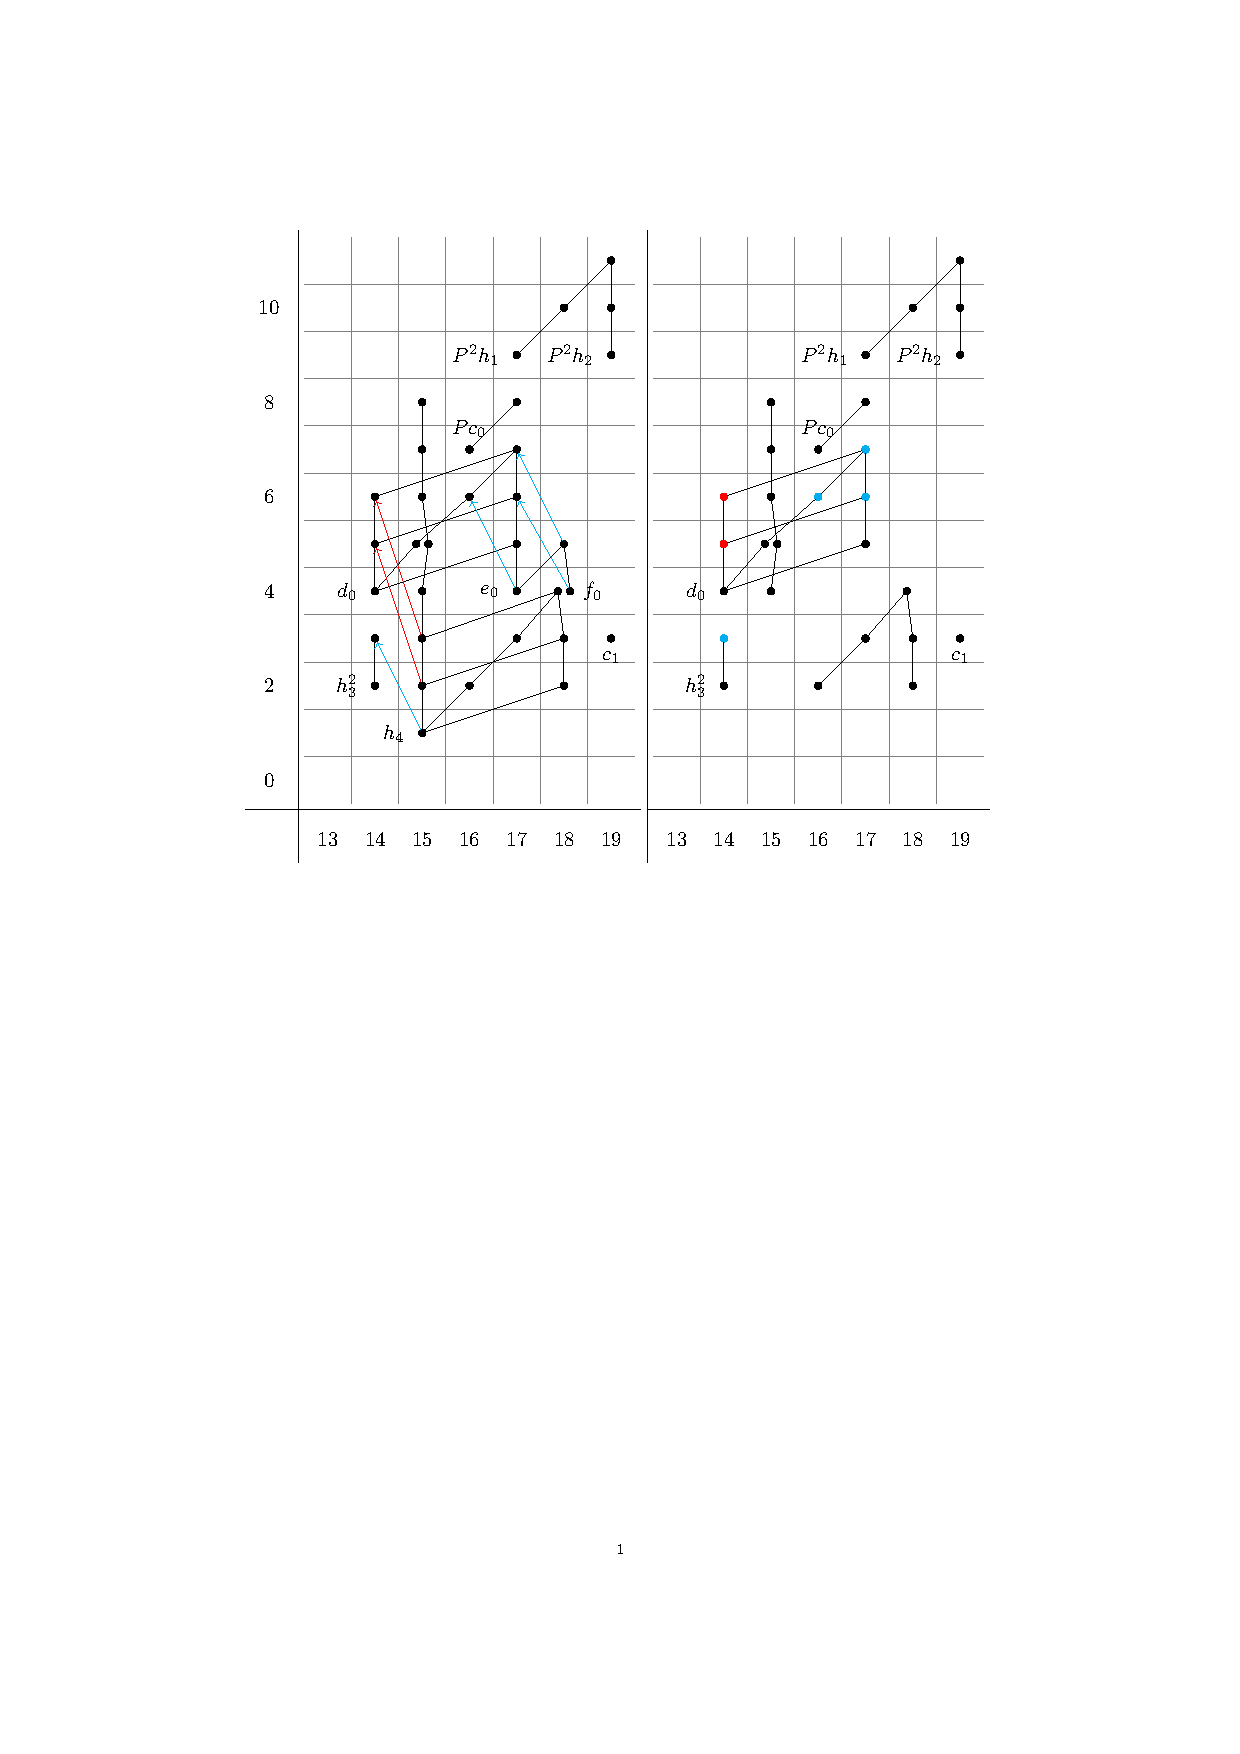
\includegraphics[trim={3.9cm 15.2cm 3.9cm 4cm}, clip, scale=1]{bleh2.pdf}
  %\printpage[ name = ASS, page = 2 ]
  %\printpage[ name = ASS, page = 3, no y ticks, x axis tail = 0cm ]
   \caption{Left: Adams spectral sequence for the sphere, with differentials color-coded by length. Right: $\mathrm{E}_\infty$-page of the synthetic Adams spectral sequence for $\nu_{\HFt} \Ss_2^\wedge$. Black dots indicate a copy of $\F_2[\tau]$, red dots indicate a copy of $\F_2[\tau]/\tau^2$ and blue dots indicate a copy of $\F_2[\tau]/\tau$.}
   \label{fig:syn-toda-range-sseq}
\end{figure}

Before proving \Cref{prop:syn-toda-range} we discuss some of the subtleties which appear in this range.
The results of this proposition are also summarized in \Cref{fig:syn-toda-range}.

\begin{rmk} \label{rmk:subtle-mult}
  The first hidden extension in the Adams spectral sequence occurs in stem 9 where on the $\mathrm{E}_2$-page $h_2^3 = h_1^2h_3$ but in homotopy $\nu^3 = \eta^2\sigma + \eta\epsilon$. Synthetically the presence of this hidden term is reflected by the appearance of a $\tau$ in relation (3) where
  \[ \wt{\nu}^3 = \wt{\eta}^2 \wt{\sigma} + \tau \wt{\eta} \wt{\epsilon}. \]

  Similarly in stem 16 the hidden extension from $h_0^3h_4$ to $Pc_0$ is reflected by relation (2) where $ \wt{\eta} \wt{\rho}  = \tau^2 \wt{Pc_0} $. Note that in this case the multiplication jumps by 2 Adams filtrations and therefore 2 $\tau$'s appear in the product. This product relation is depicted by the green line originating from $\wt{\rho}$ in \Cref{fig:syn-toda-range}

  Another subtlety is that products that are classically zero need not be zero synthetically (though they will be $\tau$-power torsion). In this range the key example of this is relation (14) where $\wt{2}^2 \wt{\sigma}^2 = \tau \wt{2} \wt{\kappa}$. In this relation we see a product which is $\tau$-torsion hidden extend to a $\tau^2$-torsion class and it is depicted by the bent green line in \Cref{fig:syn-toda-range}. A combination of these features appears in relation (15). 
\end{rmk}


\begin{rmk}
In \Cref{prop:syn-toda-range} the generators are chosen using \Cref{thm:synthetic-Adams}(3).
It is important to note that there are ambiguities in this notation.
For some classes $\wt{x}$, $x$ refers to an element of the homotopy $\Ss^{\wedge}_2$.  In these cases $\wt{x}$ is determined up to $\tau$-power torsion classes of higher $\nu \HFt$-Adams filtration.
For other classes $\wt{x}$, $x$ refers to a permanent cycle on the $\mathrm{E}_2$-page of the Adams spectral sequence for $\Ss^{\wedge}_2$.  These classes are only determined up to elements of higher $\nu \HFt$-Adams filtration.  However, in the case that $x$ is the target of a $d_{m+1}$-differential, we more precisely define $\wt{x}$ up to elements of higher $\nu \HFt$-filtration which are $\tau^m$-torsion.
%(we set $m = \infty$ if it is nonzero on the $\mathrm{E}_\infty$-page) then $\wt{x}$ is defined up to elements of higher $\nu \HFt$-filtration which are $\tau^m$-torsion.

In particular, note that the classes $\wt{2}$, $\wt{\eta}$ and $\wt{\nu}$ are unambiguously determined. On the other hand, one could, for example, replace $\wt{\kappa}$ with $3\wt{\kappa}$ or $\wt{c_1}$ with $\wt{c_1} + a\tau^6 \wt{P^2h_2}$. Nevertheless, we claim that the proposition is valid for any collection of generators provided by \Cref{thm:synthetic-Adams}(3) \emph{as long as we choose a $\wt{c_1}$ which is 2-torsion.}
\end{rmk}

\begin{rmk}
It is also important to note that multiplication may not interact nicely with the tilde notation: $\wt{x} \wt{y}$ might not be a valid choice of representative for $\wt{xy}$ since $\wt{x}\wt{y}$ may not satisfy the $\tau$-torsion requirement that \Cref{thm:synthetic-Adams}(3) places on $\wt{xy}$. However, it is true that $\wt{x} \wt{y} - \wt{xy}$ is divisible by $\tau$, and often this can be used to show that $\wt{x}\wt{y}$ does in fact satisfy the $\tau$-torsion requirement.

Furthermore, when solving extension problems one needs to be careful about exactly which bigraded homotopy elements one chooses. For example, both $\wt{\sigma}^2$ and $\wt{\sigma}^2 + \tau^2 \wt{\kappa}$ are valid choices of $\wt{h_3^2}$, but $\wt{\eta} \wt{\sigma}^2 = 0$ whereas $\wt{\eta} (\wt{\sigma}^2 + \tau^2 \wt{\kappa}) = \tau^2 \wt{\eta} \wt{\kappa} \neq 0$.
\end{rmk}

%% \newpage

\begin{figure}
  \centering
  $\pi_{k,k+s} \nu_{\HFt} (\Ss^{\wedge} _2)$ for $13 \leq k \leq 19$
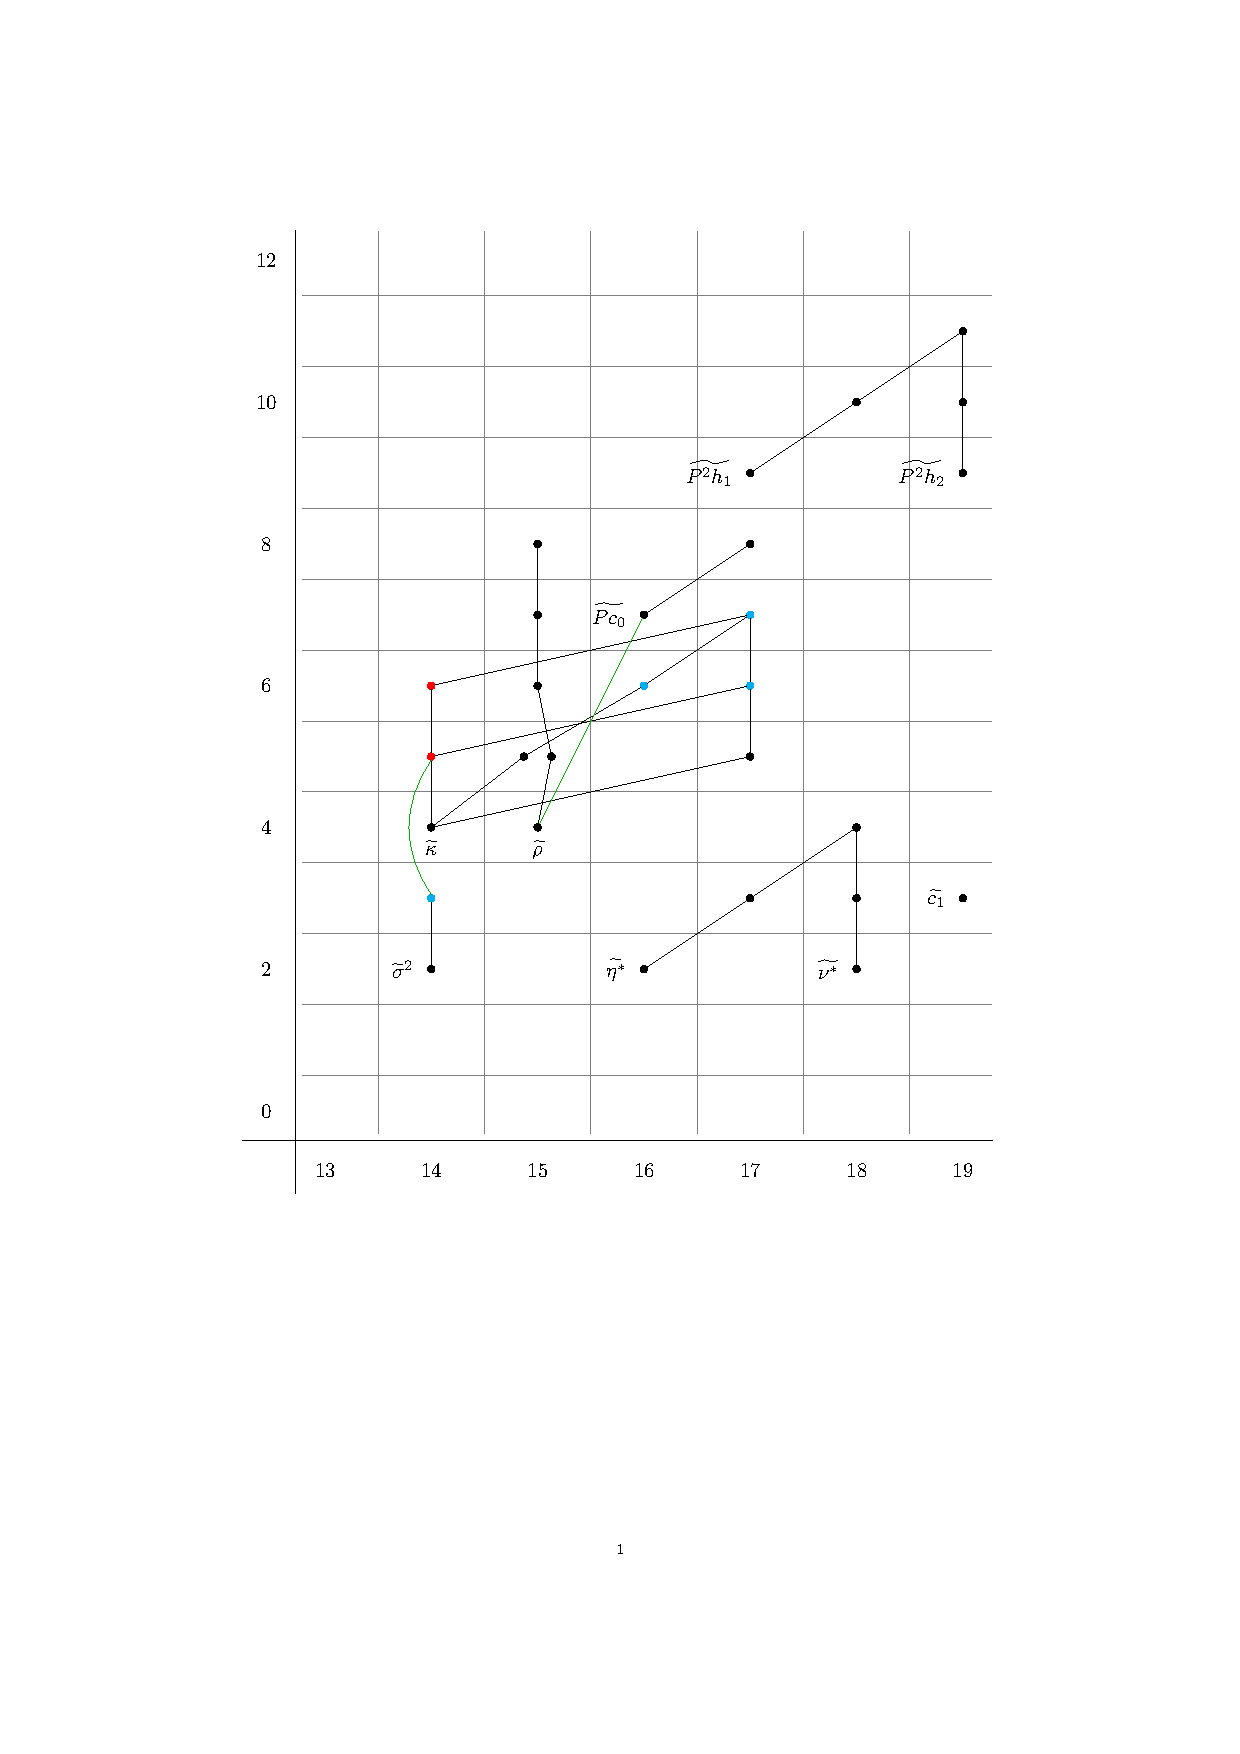
\includegraphics[trim={3.8cm 9.6cm 3.8cm 5cm}, clip, scale=1]{bleh1.pdf}
  \caption{A picture of $\pi_{k,*}$ for $13 \leq k \leq 19$. We index the picture so that bidegree $(k,k+s)$ corresponds to position $(k,s)$.
    Black dots indicate non-$\tau$-torsion classes,
    red dots indicate $\tau^2$-torsion and
    blue dots indicate $\tau$-torsion.
    We suppress all $\tau$-multiples in this figure.
    Black lines correspond to $\wt{2}$, $\wt{\eta}$ and $\wt{\nu}$ multiplications which are detected at the level of $C\tau$.
    Green lines are used for more complicated $\wt{2}$ and $\wt{\eta}$ multiplications.
    In this range the green line indicate a multiplication which hits a power of $\tau$ times the indicated dot (see \Cref{rmk:subtle-mult} for further discussion).
    }
  \label{fig:syn-toda-range}
\end{figure}



%% \begin{comment}
%% \begin{figure}
%%   \centering
%%   $\pi_{k,k+s} \nu_{\HFt} (\Ss^{\wedge} _2)$ for $13 \leq k \leq 19$
%%   \begin{sseqpage}[ xscale=1.8, yscale=1.2, x range = {13}{19}, y range = {0}{12}, x tick step = 1, y tick step = 2, class labels = {left}, classes = fill, grid = crossword ]
%%     \class["\wt{\sigma}^2"](14,2) \class[cyan](14,3) \structline

%%     \class["\wt{\kappa}"](14,4)
%%     \foreach \i in {1,...,5} { \class(14, 4 - \i) \structline[red] }
%%     \class[red](14,5) \structline(14,4) \class[cyan](14,4) \structline[red] \structline(14,3,2)
%%     \class[red](14,6) \structline(14,5) \class[cyan](14,5) \structline[red] \structline(14,4,2)
%%     \structline[green](14,3,1)(14,4,2)
    
%%     \class(15,5) \structline(14,4,1) \class[cyan](16,6) \structline
%%     \class(17,5) \structline(14,4,1) \class[cyan](17,6) \structline \structline(14,5,1)
%%     \class[cyan](17,7) \structline(14,6) \structline(16,6) \structline
  
%%     \class["\wt{\rho}" {below=0.2em}](15,4)
%%     \foreach \i in {5,...,8} { \class(15, \i) \structline }
    
%%     \class["\wt{\eta^*}"](16,2) \class(17,3) \structline
%%     \class["\wt{\nu^*}"](18,2) \class(18,3) \structline 
%%     \class(18,4) \structline(17,3) \structline
  
%%     \class["\wt{Pc_0}"](16,7)
%%     \foreach \i in {1,...,7} { \class(16, 7 - \i) \structline[red] }
%%     \structline[green](15,4)(16,5)

%%     \class(17,8) \structline(16,7)

%%     \class["\wt{P^2h_1}"](17,9) \class(18,10) \structline
%%     \class["\wt{P^2h_2}"](19,9) \class(19,10) \structline
%%     \class(19,11) \structline(18,10) \structline
%%     \class["\wt{c_1}"](19,3)
%%   \end{sseqpage}

%%   \caption{A picture of $\pi_{k,*}$ for $13 \leq k \leq 19$. We index the picture so that bidegree $(k,k+s)$ corresponds to position $(k,s)$.
%%     Black dots indicate non-$\tau$-torsion classes,
%%     red dots indicate $\tau^2$-torsion and
%%     blue dots indicate $\tau$-torsion.
%%     Black lines correspond to $\wt{2}$, $\wt{\eta}$ and $\wt{\nu}$ multiplications which are detected in the $\nu \HFt$-Adams spectral sequence. Red lines correspond to $\tau$ multiplications, and green lines correspond to hidden $\wt{2}$ and $\wt{\eta}$ extensions.
%%     We suppress all $\tau$-multiples except those which take part in hidden extensions.
%%     Note that the blue dot in $(14,4)$ is $2 \wt{\kappa}$  because of the relation $2 = \tau \wt{2}$.}
%% \end{figure}
%% \end{comment}

\begin{proof}
  Using \Cref{thm:synthetic-Adams} we may produce the generators listed above.
  This theorem also lets us conclude that the $\tau$-adic completion of the algebra they generate is equal to $\pi_{k,*}$ for $k \leq 19$.

  Before we continue we use \Cref{cor:tau-torsion-bound} to find which bigraded groups have $\tau$-power torsion elements. The only bigraded groups with $k \leq 19$ for which $\pi_{k,k+s}^{\mathrm{tor}}$ is nonzero are
  $$ \pi_{14,17},\ \pi_{14,18},\ \pi_{14,19},\ \pi_{14,20},\ \pi_{16,22},\ \pi_{17,23},\ \pi_{17,24}. $$
  This means that $\tau^{-1} : \pi_{k,k+s} \to \pi_k$ is an inclusion in all other bidegrees.
  Moreover, since the functor $\tau^{-1}$ is symmetric monoidal, it follows that these inclusions respect the multiplicative structure on both sides. Thus, we may deduce that (0)--(9) follow from the associated relations in usual homotopy groups.

  To prove the relation (10), note that the element $\wt{\sigma}$ lives in an odd topological degree. Therefore, we learn that $2 \wt{\sigma}^2 = 0$ by considering the $\mathbb{E}_\infty$-ring structure on $\nu_{\HFt}(\Ss_2^\wedge)$ (see \cite[Remark 4.10]{Pstragowski}). 

  Relations (11) and (12) follow from the fact that both $\eta^2\kappa$ and $2\nu\kappa$ are zero in the usual homotopy groups of $\Ss_2^{\wedge}$.  Therefore both $\wt{\eta}^2\wt{\kappa}$ and $\wt{2}\wt{\nu}\wt{\kappa}$ are $\tau$-power torsion.  Since they live in bidegrees containing only simple $\tau$-torsion, it follows that $\tau$ times them is zero.  Note that $\tau \wt{2}\wt{\nu}\wt{\kappa}=2 \wt{\nu}\wt{\kappa}$.

  To prove (13) and (15) we consider the ring map
  $$ \nu_{\HFt}(\Ss^\wedge_2) \to C\tau \otimes \nu_{\HFt}(\Ss^\wedge_2). $$
  Because there are no $\tau$-power torsion elements which are also divisible by $\tau$ in $\pi_{14,20}$ or $\pi_{16,22}$, this map induces isomorphisms
  $$ \pi_{14,20}^{\mathrm{tor}} \cong \Ext^{6,20}_{\A_*}(\F_2, \F_2)\ \ \text{ and }\ \ \pi_{16,22}^{\mathrm{tor}} \cong \Ext^{6,22}_{\A_*}(\F_2, \F_2). $$
  Thus, once we know that each term is zero in the usual homotopy groups we can read (13) and (15) off from the corresponding relation in the $\mathrm{E}_2$ page.

  In the Toda range (14) is the most difficult relation.
  To obtain it, we will make use of the long exact sequence
  \begin{center}
    \begin{tikzcd}
      \cdots \ar[r] &
      \pi_{k+1,k+s-1} \ar[r] \arrow[draw=none]{d}[name=Z, shape=coordinate]{} &
      \Ext^{s-2,k+s-1}_{\A_*}(\F_2, \F_2) \arrow[rounded corners,to path={ -- ([xshift=2ex]\tikztostart.east)|- (Z) [near end]\tikztonodes-| ([xshift=-2ex]\tikztotarget.west)-- (\tikztotarget)}]{dl} & \\
        &
      \pi_{k,k+s} \ar[r, "\cdot \tau"] &
      \pi_{k,k+s-1} \ar[r] &
      \cdots.
    \end{tikzcd}
  \end{center}
  From (10) and the torsion bound on $\pi_{14,18}$ we know that $\wt{2} \wt{\sigma}^2$ and $2 \wt{\kappa}$ are both simple $\tau$-torsion. Thus, they lift to non-zero classes in $\Ext^{1,16} _{\A_*} (\F_2, \F_2)$ and $\Ext^{2,17} _{\A_*} (\F_2, \F_2)$, respectively. These classes must be $h_4$ and $h_0 h_4$, and hence are related by multiplication by $h_0$.
	This implies that their images are related by multiplication by $\wt{2}$, as desired.

    Finally, using parts (2a), (3a), (3b) and (4) of \Cref{thm:synthetic-Adams}, one may compute the length of $\pi_{k,k+s}$ as a $\Z_2$-module for each $k \leq 19$ and all $s$. From this we may conclude that there are no further relations for size reasons.
\end{proof}


%%% Local Variables:
%%% mode: latex
%%% TeX-master: "Main"
%%% eval: (visual-line-mode t)
%%% eval: (auto-fill-mode 0)
%%% End:
